
\subsection{Overview of Historical Survey} \label{sec:survey-overview}
%To better document these programs, we rely on data from the historical survey, reported by local experts in Reggio Emilia (municipal and state only); in Parma (municipal only); and in Padova (municipal, state, and religious).

%NOTE: PLEASE KEEP THE PARAGRAPH BELOW 
Other early childhood education systems within Reggio Emilia, as well as in Parma and Padova, share certain features of program administration, practices for at-risk children and families, and pedagogical methods. However, Published literature about the municipal early childhood systems in Parma and Padova is scarce. To better compare these systems, we administered a historical survey to current and retired school administrators and educative coordinators from each system in each city. Survey responses were received from the following systems that allowed us to document the history of early childhood programming in each municipality: in Reggio Emilia, municipal and state; in Parma, municipal; and in Padova, municipal, state, and religious. Responses were also received from religious systems in Reggio Emilia and in Parma, however, they did not include historical data prior to 2000. 

%\noindent\textbf{[YKK: I think since the tables show what questions were asked, it may be better to move the list of all questions to the appendix and just explain them briefly in the main paper, which I did. What do you think? SK: Noted, and I edited the text somewhat.]}
The historical survey is designed to compare administrative and pedagogical components present in the Reggio Approach with each of the other systems. The survey was developed based on published program descriptions, and confirmed by expert scholars with firsthand knowledge of the Reggio Approach and early childhood programs in northern Italy.\footnote{See \citet{Edwards-etal-eds_1998_Hundred-Languages} and \citet{Corsaro_2008_Policy-Practice}.} The questionnaire includes administrative program operations including staffing, supervision, enrollment, and funding. It also considers pedagogy and educational practices for children's learning in various dimensions. For a more detailed summary of questions, see Appendix \ref{sec:survey}.

%\subsubsection{Enrollment in Early Childhood Systems}

%Figure \ref{fig:enrollment} explores the similarities and difference in enrollment statistics in each of the three cities \citep{Padova-Admin-Data_1964-2011,Reggio-Admin-data_1966-2006,Reggio-Annual-Journals_1994-2011}. Note that enrollment data is not available for Parma except for the year 2010. 

%Historically, Padova demonstrates the highest rate of preschool attendance. We also see that Reggio Emilia and Padova observed increases in preschool enrollment; by the 1990s, almost all eligible children are enrolled in preschool. Trends in municipal preschool enrollment demonstrate an increase during the 1970s and the 1980s in Reggio Emilia and Padova. Historically, in both Reggio Emilia and Padova, state preschool enrollments increased whereas religious preschool enrollment decreased. In Parma, enrollment statistics in 2010 are similar to those of Reggio Emilia. 

%\begin{figure}[H]
%      \centering
%        \begin{subfigure}[t]{0.49\textwidth}
%          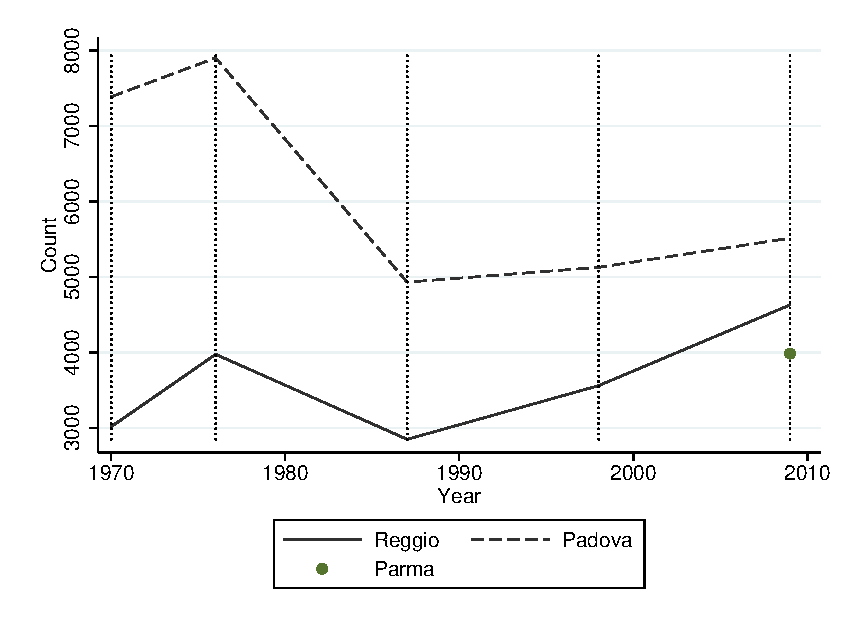
\includegraphics[width=\textwidth]{../../output/image/enroll_num_graph.eps}       
%\caption{Num. of Children Enrolled in Preschool}        
%        \end{subfigure}
%        \begin{subfigure}[t]{0.49\textwidth}
%          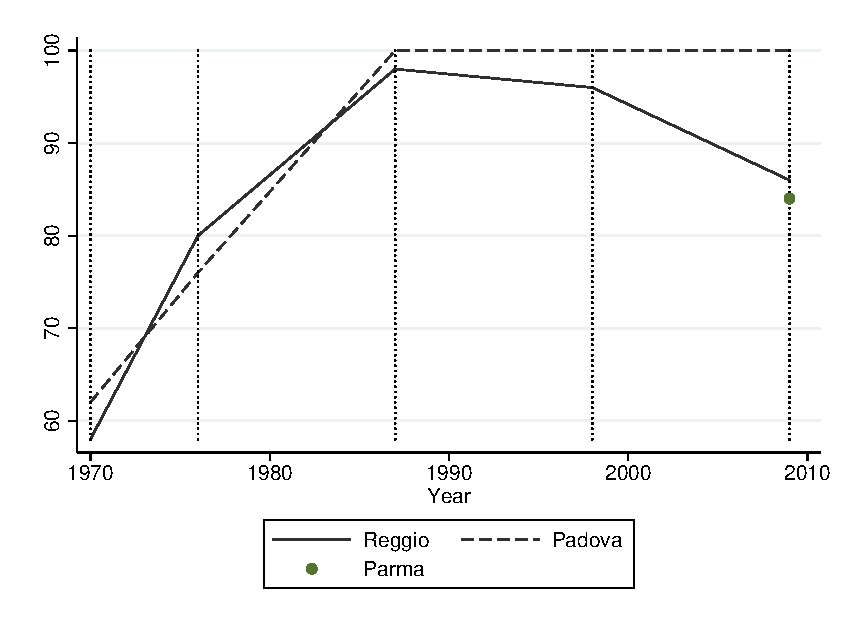
\includegraphics[width=\textwidth]{../../output/image/enroll_per_graph.eps}       
% \caption{Percentage of Ages 3-5 Enrolled in Preschool}        
%        \end{subfigure}
%        \begin{subfigure}[t]{0.49\textwidth}
%          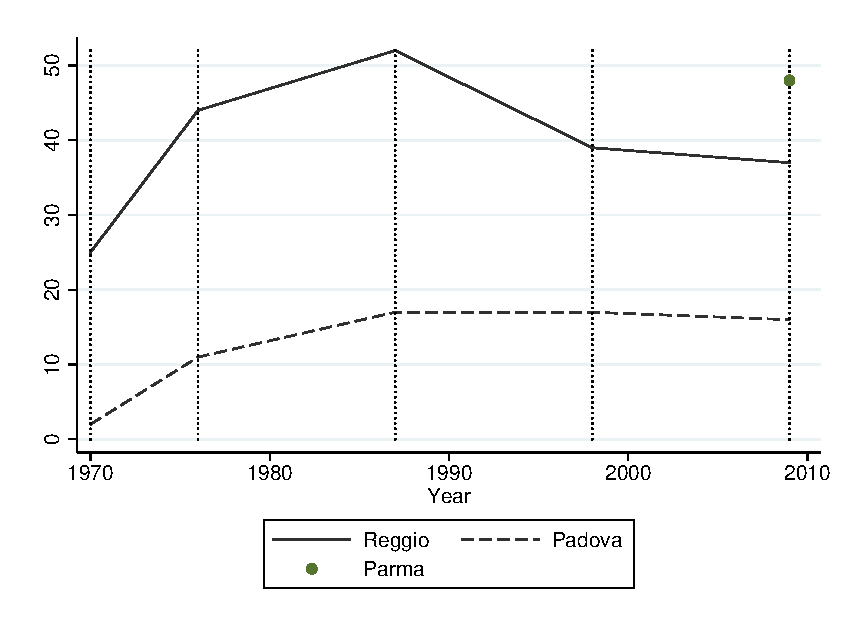
\includegraphics[width=\textwidth]{../../output/image/enroll_per_muni_graph.eps} 
%        \caption{Percentage of Enrollment in Municipal Preschools}        
%        \end{subfigure}
%        \begin{subfigure}[t]{0.49\textwidth}
%          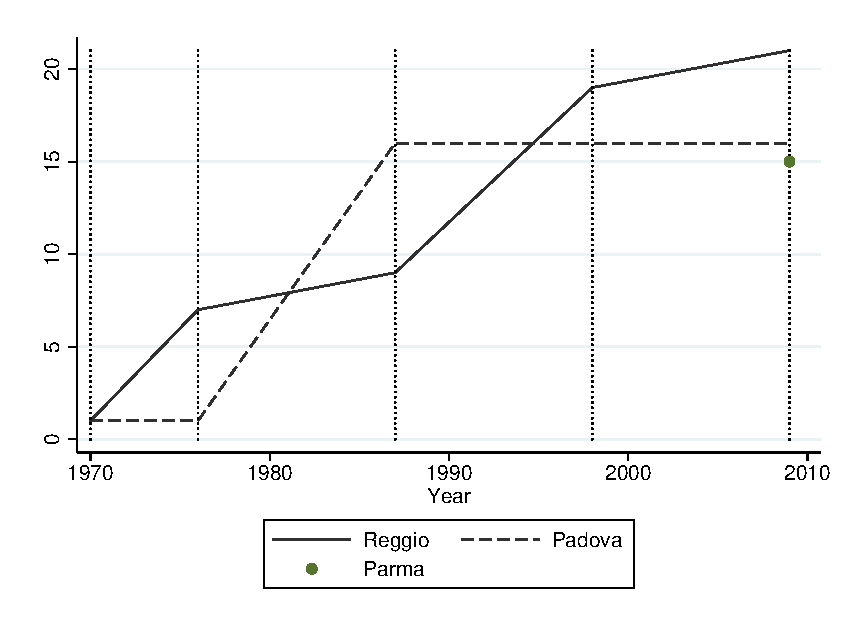
\includegraphics[width=\textwidth]{../../output/image/enroll_per_stat_graph.eps}
%            \caption{Percentage of Enrollment in State Preschools}       
%        \end{subfigure}
%      \begin{subfigure}[ht]{0.48\textwidth}
%        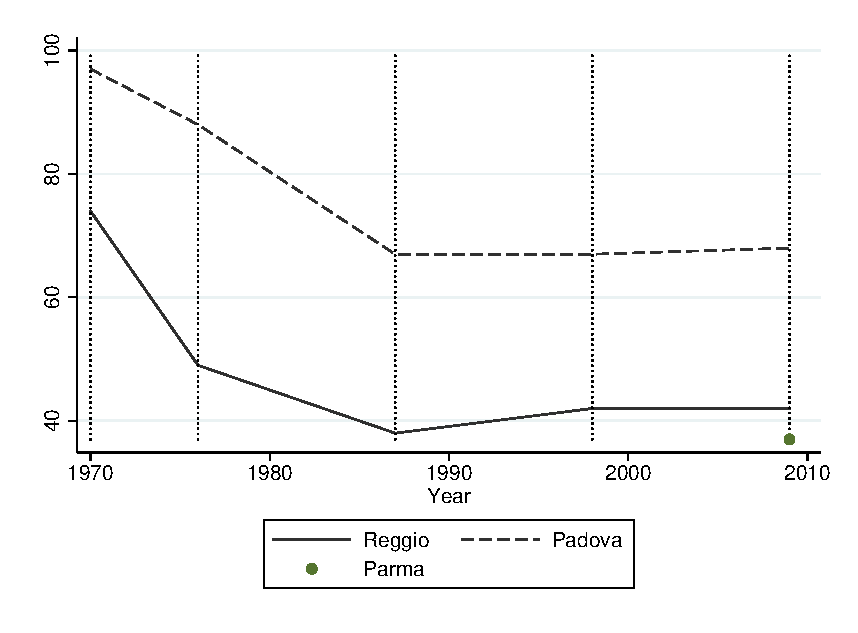
\includegraphics[width=\textwidth]{../../output/image/enroll_per_priv_graph.eps}
%        \caption{Percentage of Enrollment in Religious Preschools}
  %      \label{fig:large}
 %     \end{subfigure}
%      \caption{Enrollment Statistics}  %\label{fig:enrollment}
%    \end{figure}

\subsection{Results of the Historical Survey}

The historical survey demonstrates similarities and differences in administrative and pedagogical components between the Reggio Approach and alternative treatments. Results from the historical survey indicate that early childhood education systems within Reggio Emilia, as well as in Parma and Padova, share certain features of program administration, practices for at-risk children and families, and pedagogical methods. The general trend shows that the components endorsed by the Reggio Approach are increasingly present in other systems, albeit in different degrees. We interpret the results from the historical survey as evidence for potential spillovers into alternative treatments; it is widely accepted that Malaguzzi and other Reggio Emilia municipal leaders influenced ongoing state policies and legislation. 



To summarize, we present the similarities and differences between the different programs in Figures~\ref{fig:agg-admin} and~\ref{fig:agg-ped}. Using results from the structured interviews, we compute the number of administrative and pedagogical components that each program shares with the Reggio Approach by school type, city, and year. We examine 14 administrative components and 16 pedagogical components (not all of the pedagogical components were present in the Reggio Approach). Over time, many of the programs other than the state programs, adopted more features present in the Reggio Approach. This is especially true of the Parma municipal program when examining administrative components. The other programs did not adopt as many pedagogical components as they did administrative ones. Even though the Reggio Approach remained distinctive when considering the sum of its elements, many of the alternative schools evolved to include certain elements.

\begin{figure}[H]
\begin{center}
\begin{subfigure}[b]{0.49\textwidth}
	\caption{Number of Administrative Characteristics in Common with the Reggio Approach}\label{fig:agg-admin}
	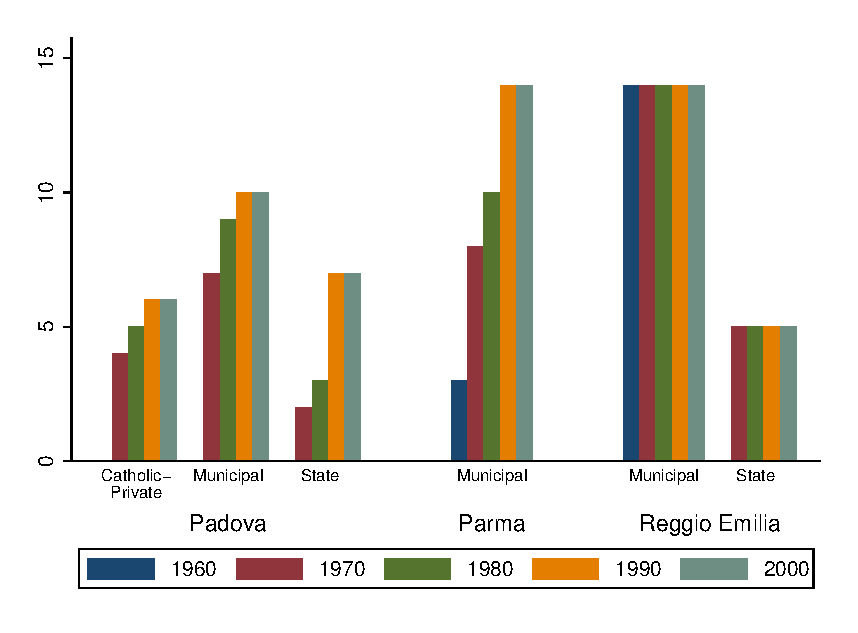
\includegraphics[width=\textwidth]{../../output/aggregateAdministrative.eps}
\end{subfigure}%
~
\begin{subfigure}[b]{0.49\textwidth}
	\caption{Number of Pedagogical Characteristics in Common with the Reggio Approach}\label{fig:agg-ped}
	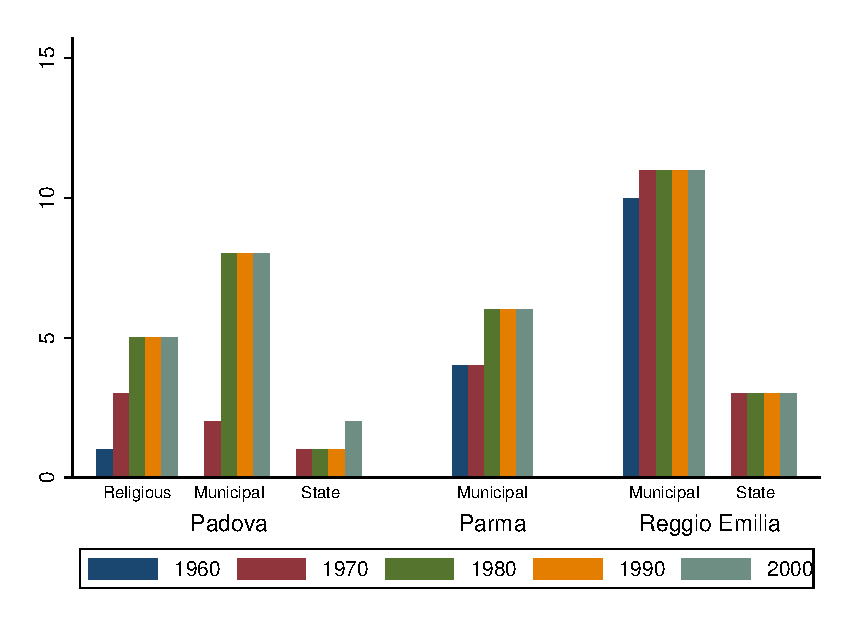
\includegraphics[width=\textwidth]{../../output/aggregatePedagogical.eps}
\end{subfigure}%
\end{center}
\raggedright \footnotesize Note: These graphs show the number of administrative and pedagogical components that each program has in common with the Reggio Approach. We consider 14 administrative components and 16 pedagogical components. Some of the pedagogical components were not present in the Reggio Approach. 
\end{figure}

We emphasize the results of the survey for items that are related to prioritizing disadvantaged children. Municipal schools in the three cities shared priorities of enrolling economically disadvantaged children, children from a single-parent household, and children with disabilities.


Results for administrative operations of early childhood system from 1960 through 2010 against systematic features of Reggio Emilia's municipal program are shown in Table \ref{tab:programoperation}. We find that each of the municipalities, state, and religious systems invested in early childhood programming in different times and in different ways. We find innovation in the Reggio Approach and considerable investment by the Reggio Emilia municipality in a large and comprehensive early childhood system as well as in local state and religious preschools. Table \ref{tab:programoperation} demonstrates that municipal programs in Parma and Padova contain more features of program operations endorsed by the Reggio Approach than other types of programs do, especially after the 1990s.

Results for administrative practices for at-risk children and families in each early childhood system from 1960 through 2010 relative to Reggio Emilia's municipal program are presented in Table \ref{tab:administrative-atrisk}. The hours of center-based care is largely shared by the surveyed programs. All systems (except the state preschools in Padova) offered additional hours for working families. Similarly, by the 1990s, all surveyed systems received public funding. Municipal schools in the three cities shared priorities of enrolling economically disadvantaged children, children from a single-parent household, and children with disabilities.							

Educational programming in each early childhood system from 1960 through 2010 against systematic features of Reggio Emilia's municipal program is reported in Table \ref{tab:educ-program}. Municipal systems in three cities after the 1990s all endorse theory-based curricula, require teachers to document children's learning, and are influenced by academic theories of psychology and early childhood interventions. We recognize the availability of early childhood experts to Parma and Padova in the presence of respected scholars from local universities. For example, municipal systems in Parma and Padova implement daily activities that guide children in learning specific concepts and provide religious teaching, both of which are not present in the Reggio Approach. The state systems in Reggio Emilia and Padova appear to share very little of the educational components present in the Reggio Approach.												

Environmental components of early childhood system from 1960 through 2010 relative to systematic features of Reggio Emilia's municipal program are report in Table \ref{tab:environ-features}. Municipal systems in three cities are shown to share similar environmental features, such as the presence of Atelier and open spaces.   
				
				
To summarize, municipal systems in Reggio Emilia, Parma, and Padova share similar components in program operations, administrative practices for at-risk children, educational programming, and environmental features. 

%\textbf{[YKK: I think more summary description is needed for difference between the Reggio Approach and Reggio state, Padova state, Padova religious, municipal-affiliated (in general), because they appear in the later sections. I also think it may be better to briefly explain why Reggio religious and Parma Religious and State are not included in the survey. I think we might need to (1) acknowledge that we are not able to get enough information about schools not surveyed and the reasons why and (2) briefly explain the differences between Reggio Approach and the systems that are not surveyed.]}			
